\documentclass[aspectratio=169]{beamer}

\usepackage{amsmath}
\usepackage{booktabs}
\usepackage[table]{xcolor}
\usepackage{tikz}
\usetikzlibrary{arrows.meta,positioning,calc}
\usepackage{array}

\title{Worker Productivity and Plant Fixed Effects}
\author{}
\date{}

%----------------------------------
% Elegant visual system
\definecolor{DeepNavy}{HTML}{102A43}
\definecolor{Slate}{HTML}{334E68}
\definecolor{SoftBlue}{HTML}{EAF2F8}
\definecolor{SoftTeal}{HTML}{E6FFFA}
\definecolor{AccentTeal}{HTML}{0F766E}
\definecolor{AccentGold}{HTML}{B7791F}
\definecolor{SoftGold}{HTML}{FFF7E6}
\definecolor{SoftGray}{HTML}{F6F8FA}
\definecolor{LineGray}{HTML}{CBD5E1}
\definecolor{Positive}{HTML}{0F766E}
\definecolor{Negative}{HTML}{B91C1C}

\usetheme{default}
\usefonttheme{professionalfonts}
\setbeamercolor{normal text}{fg=DeepNavy,bg=white}
\setbeamercolor{frametitle}{fg=white,bg=DeepNavy}
\setbeamercolor{title}{fg=white,bg=DeepNavy}
\setbeamercolor{subtitle}{fg=white,bg=DeepNavy}
\setbeamercolor{structure}{fg=AccentTeal}
\setbeamercolor{bluebox}{fg=DeepNavy,bg=SoftBlue}
\setbeamercolor{tealbox}{fg=DeepNavy,bg=SoftTeal}
\setbeamercolor{goldbox}{fg=DeepNavy,bg=SoftGold}
\setbeamercolor{graybox}{fg=DeepNavy,bg=SoftGray}

\setbeamertemplate{navigation symbols}{}
\setbeamertemplate{itemize item}{\color{AccentTeal}$\blacktriangleright$}
\setbeamertemplate{itemize subitem}{\color{AccentGold}$\bullet$}
\setbeamertemplate{footline}{%
  \leavevmode%
  \hbox{%
  \begin{beamercolorbox}[wd=.72\paperwidth,ht=2.4ex,dp=1.1ex,leftskip=.45cm]{graybox}%
    \scriptsize Worker Productivity and Plant Fixed Effects
  \end{beamercolorbox}%
  \begin{beamercolorbox}[wd=.28\paperwidth,ht=2.4ex,dp=1.1ex,rightskip=.45cm plus1fil]{graybox}%
    \scriptsize\hfill \insertframenumber/\inserttotalframenumber
  \end{beamercolorbox}}%
}
\setbeamertemplate{frametitle}{%
  \vspace{0.12cm}
  \begin{beamercolorbox}[wd=\paperwidth,ht=0.68cm,dp=0.22cm,leftskip=0.55cm,rightskip=0.45cm]{frametitle}
    \usebeamerfont{frametitle}\insertframetitle
  \end{beamercolorbox}
  \vspace{-0.12cm}
}

\newcommand{\softbox}[2]{%
\begin{beamercolorbox}[rounded=true,shadow=false,wd=\linewidth,sep=0.18cm]{#1}
#2
\end{beamercolorbox}}

\newcommand{\tagbox}[1]{%
\tikz[baseline=(X.base)]\node[fill=SoftTeal,draw=AccentTeal!35,rounded corners=2pt,inner xsep=5pt,inner ysep=2pt](X){\scriptsize\textbf{#1}};}

\newcommand{\stepbubble}[2]{%
\begin{tikzpicture}[baseline=(n.base)]
\node[circle,fill=AccentTeal,text=white,minimum size=0.55cm,font=\bfseries\scriptsize](n){#1};
\node[right=0.12cm of n,align=left,text=DeepNavy,font=\scriptsize](t){#2};
\end{tikzpicture}}

\newcommand{\coefchartLogQuant}{%
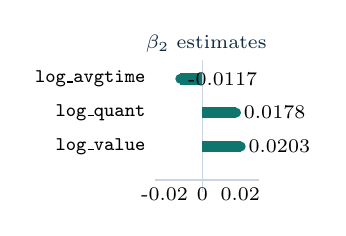
\begin{tikzpicture}[x=24cm,y=0.43cm]
\scriptsize
\draw[LineGray,thick] (-0.025,0) -- (0.030,0);
\draw[LineGray] (0,-0.35) -- (0,3.55);
\node[above,DeepNavy] at (0.002,3.55) {$\beta_2$ estimates};
\foreach \y/\lab/\val in {3/{\texttt{log\_avgtime}}/-0.0117,2/{\texttt{log\_quant}}/0.0178,1/{\texttt{log\_value}}/0.0203}{
  \node[left] at (-0.026,\y) {\lab};
  \draw[line width=4.2pt,AccentTeal] (0,\y) -- (\val,\y);
  \fill[AccentTeal] (\val,\y) circle (1.8pt);
  \node[right] at (\val,\y) {\val};
}
\node[below] at (-0.020,0) {-0.02};
\node[below] at (0,0) {0};
\node[below] at (0.020,0) {0.02};
\end{tikzpicture}}

\newcommand{\coefchartBehaviorLogQuant}{%
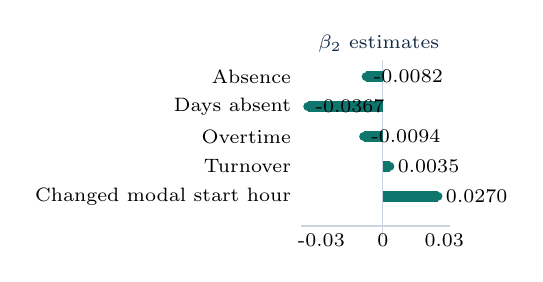
\begin{tikzpicture}[x=26cm,y=0.38cm]
\scriptsize
\draw[LineGray,thick] (-0.040,0) -- (0.033,0);
\draw[LineGray] (0,-0.35) -- (0,5.55);
\node[above,DeepNavy] at (-0.002,5.55) {$\beta_2$ estimates};
\foreach \y/\lab/\val in {5/{Absence}/-0.0082,4/{Days absent}/-0.0367,3/{Overtime}/-0.0094,2/{Turnover}/0.0035,1/{Changed modal start hour}/0.0270}{
  \node[left,align=right] at (-0.041,\y) {\lab};
  \draw[line width=3.8pt,AccentTeal] (0,\y) -- (\val,\y);
  \fill[AccentTeal] (\val,\y) circle (1.6pt);
  \node[right] at (\val,\y) {\val};
}
\node[below] at (-0.030,0) {-0.03};
\node[below] at (0,0) {0};
\node[below] at (0.030,0) {0.03};
\end{tikzpicture}}

\newcommand{\coefchartAvgtimeProductivity}{%
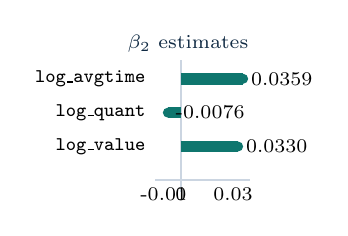
\begin{tikzpicture}[x=22cm,y=0.43cm]
\scriptsize
\draw[LineGray,thick] (-0.015,0) -- (0.040,0);
\draw[LineGray] (0,-0.35) -- (0,3.55);
\node[above,DeepNavy] at (0.004,3.55) {$\beta_2$ estimates};
\foreach \y/\lab/\val in {3/{\texttt{log\_avgtime}}/0.0359,2/{\texttt{log\_quant}}/-0.0076,1/{\texttt{log\_value}}/0.0330}{
  \node[left] at (-0.016,\y) {\lab};
  \draw[line width=4.2pt,AccentTeal] (0,\y) -- (\val,\y);
  \fill[AccentTeal] (\val,\y) circle (1.8pt);
  \node[right] at (\val,\y) {\val};
}
\node[below] at (-0.010,0) {-0.01};
\node[below] at (0,0) {0};
\node[below] at (0.030,0) {0.03};
\end{tikzpicture}}

\newcommand{\coefchartAvgtimeBehavior}{%
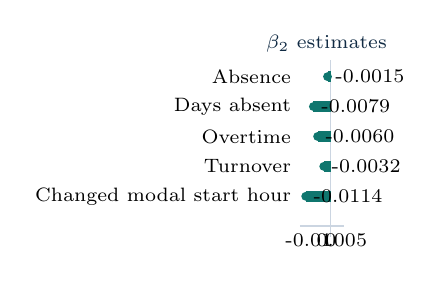
\begin{tikzpicture}[x=28cm,y=0.38cm]
\scriptsize
\draw[LineGray,thick] (-0.014,0) -- (0.006,0);
\draw[LineGray] (0,-0.35) -- (0,5.55);
\node[above,DeepNavy] at (-0.002,5.55) {$\beta_2$ estimates};
\foreach \y/\lab/\val in {5/{Absence}/-0.0015,4/{Days absent}/-0.0079,3/{Overtime}/-0.0060,2/{Turnover}/-0.0032,1/{Changed modal start hour}/-0.0114}{
  \node[left,align=right] at (-0.0145,\y) {\lab};
  \draw[line width=3.8pt,AccentTeal] (0,\y) -- (\val,\y);
  \fill[AccentTeal] (\val,\y) circle (1.6pt);
  \node[right] at (\val,\y) {\val};
}
\node[below] at (-0.010,0) {-0.01};
\node[below] at (0,0) {0};
\node[below] at (0.005,0) {0.005};
\end{tikzpicture}}

\begin{document}

%----------------------------------
\begin{frame}[plain]

\begin{tikzpicture}[remember picture,overlay]
    \fill[DeepNavy] (current page.south west) rectangle (current page.north east);
    \fill[AccentTeal!45] ($(current page.north east)+(-4.7,-1.1)$) circle (2.7cm);
    \fill[AccentGold!50] ($(current page.south west)+(2.2,1.0)$) circle (1.7cm);
    \draw[white!15,line width=0.7pt] ($(current page.west)+(0,1.1)$) -- ($(current page.east)+(0,1.1)$);
\end{tikzpicture}
\vspace{1.8cm}
\begin{center}
{\color{white}\Huge\bfseries Worker Productivity and Plant Fixed Effects}\par
\vspace{0.45cm}
{\color{white!78}\large Difference-in-differences evidence from worker moves}\par
\vspace{1.2cm}
\tagbox{AKM plant fixed effects}\hspace{0.25cm}\tagbox{Worker moves}\hspace{0.25cm}\tagbox{Panel outcomes}
\end{center}
\end{frame}

%----------------------------------
\begin{frame}{Objective}

\begin{columns}[T,onlytextwidth]
\begin{column}{0.54\textwidth}
\softbox{bluebox}{%
\textbf{Research question:}

\vspace{0.3cm}

What is the effect of moving to higher-productivity plants?
}

\vspace{0.35cm}

\softbox{goldbox}{%
\textbf{Parameter of interest:}

\vspace{0.3cm}

Effect of moving to a high-productivity plant on worker outcomes
}
\end{column}
\begin{column}{0.41\textwidth}
\softbox{tealbox}{%
\textbf{Identification idea:}
\begin{itemize}
    \item Plants differ in productivity (measured via AKM-style fixed effects)
    \item Workers move across plants
    \item Compare outcomes before and after moves
\end{itemize}
}
\end{column}
\end{columns}

\vspace{0.4cm}
\begin{center}
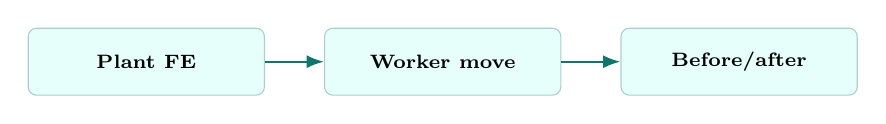
\begin{tikzpicture}[node distance=0.18cm]
\node[draw=AccentTeal!35,fill=SoftTeal,rounded corners=3pt,minimum width=3cm,minimum height=0.85cm,font=\scriptsize\bfseries] (a) {Plant FE};
\node[draw=AccentTeal!35,fill=SoftTeal,rounded corners=3pt,minimum width=3cm,minimum height=0.85cm,font=\scriptsize\bfseries,right=0.75cm of a] (b) {Worker move};
\node[draw=AccentTeal!35,fill=SoftTeal,rounded corners=3pt,minimum width=3cm,minimum height=0.85cm,font=\scriptsize\bfseries,right=0.75cm of b] (c) {Before/after};
\draw[-{Latex[length=2.2mm]},thick,AccentTeal] (a) -- (b);
\draw[-{Latex[length=2.2mm]},thick,AccentTeal] (b) -- (c);
\end{tikzpicture}
\end{center}

\end{frame}

%----------------------------------

\begin{frame}{Empirical Strategy}

\begin{columns}[T,onlytextwidth]
\begin{column}{0.49\textwidth}
\softbox{bluebox}{%
\stepbubble{1}{\textbf{Plant productivity}}

\begin{itemize}
    \item Estimate plant fixed effects (AKM framework)
        \begin{itemize}
\item Productivity measure: Log of daily quantity output %Change wording to be more clear about tickets~orders/operations, qty= number of tickets-- Log of daily orders completed
\end{itemize}

    \item Define high-productivity plants:
    \begin{itemize}
        \item Above-median plant fixed effect
    \end{itemize}
\end{itemize}
}
\end{column}
\begin{column}{0.49\textwidth}
\softbox{tealbox}{%
\stepbubble{2}{\textbf{Construct panel dataset}}

\begin{itemize}
    \item Track workers before and after plant moves
    \item Define:
    \begin{itemize}
        \item $post_{it}$: after move
        \item $high_i$: destination plant is high-FE
    \end{itemize}
\end{itemize}
}
\end{column}
\end{columns}

\vspace{0.45cm}
\begin{center}

\begin{tikzpicture}
\node[draw=LineGray,fill=white,rounded corners=3pt,minimum width=10.8cm,minimum height=1.0cm] (p) {};
\node[font=\scriptsize\bfseries,DeepNavy] at (-4.2,0) {Estimate FE};
\node[font=\scriptsize\bfseries,DeepNavy] at (-1.2,0) {Classify plants};
\node[font=\scriptsize\bfseries,DeepNavy] at (1.8,0) {Track movers};
\node[font=\scriptsize\bfseries,DeepNavy] at (4.5,0) {Define treatment};
\draw[-{Latex[length=2.2mm]},thick,AccentTeal] (-3.35,0) -- (-2.15,0);
\draw[-{Latex[length=2.2mm]},thick,AccentTeal] (-0.25,0) -- (0.90,0);
\draw[-{Latex[length=2.2mm]},thick,AccentTeal] (2.65,0) -- (3.55,0);
\end{tikzpicture}
\end{center}

\end{frame}

\begin{frame}{Empirical Strategy}

\softbox{bluebox}{%
\textbf{Step 3: Estimation of DiD model}

\[
Y_{it} = \beta_1 post_{it} + \beta_2 (post_{it} \times high_i) + \alpha_i + \gamma_t + \varepsilon_{it}
\]
}

\vspace{0.35cm}

\begin{columns}[T,onlytextwidth]
\begin{column}{0.48\textwidth}
\softbox{graybox}{%
\begin{itemize}
\item $Y_{it}$: log of the outcome value of worker $i$ at week $t$
    \item $\alpha_i$: worker fixed effects
    \item $\gamma_t$: week fixed effects
    \item Standard errors clustered at worker level %Verify standard errors for that regrssion was clustered at worker level
\end{itemize}
}
\end{column}
\begin{column}{0.48\textwidth}
\softbox{goldbox}{%
\textbf{Interpretation}
\begin{itemize}
    \item $\beta_1$: effect of movement to another plant
    \item $\beta_2$: differential effect between high- and low productivity destination plants
\end{itemize}
}
\end{column}
\end{columns}
\end{frame}
%----------------------------------

\begin{frame}{Interpretation}

\begin{columns}[T,onlytextwidth]
\begin{column}{0.55\textwidth}
\softbox{bluebox}{%
\textbf{Coefficient of interest}

\vspace{0.2cm}

\[
\beta_2 = 
\text{(High-FE movers post)} - \text{(Low-FE movers post)}
\]
}

\vspace{0.25cm}

\softbox{graybox}{%
\begin{itemize}
\item Effect of moving to a high-productivity plant
    \item Controls for worker ability (worker FE)
    \item Controls for aggregate shocks (time FE)
\end{itemize}
}
\end{column}
\begin{column}{0.41\textwidth}
\softbox{tealbox}{%
\textbf{Outcome categories}
\begin{itemize}
    \item Productivity: total quantity transported, total value transported (price plus quantity), and average time per order %Total orders completed, avg value transported per order, average time per order
    \item Behavioral: absenteeism, schedules, overtime, and turnover
\end{itemize}
}
\end{column}
\end{columns}

\vspace{0.35cm}
\begin{center}
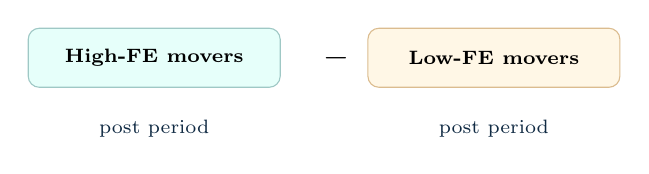
\begin{tikzpicture}
\node[draw=AccentTeal!40,fill=SoftTeal,rounded corners=4pt,minimum width=3.2cm,minimum height=0.75cm,font=\scriptsize\bfseries] (h) {High-FE movers};
\node[draw=AccentGold!50,fill=SoftGold,rounded corners=4pt,minimum width=3.2cm,minimum height=0.75cm,font=\scriptsize\bfseries,right=1.1cm of h] (l) {Low-FE movers};
\node[font=\bfseries\large,right=0.42cm of h] {$-$};
\node[font=\scriptsize,DeepNavy,below=0.28cm of h] {post period};
\node[font=\scriptsize,DeepNavy,below=0.28cm of l] {post period};
\end{tikzpicture}
\end{center}

\end{frame}

%----------------------------------
\begin{frame}{Productivity Results: Treatment Defined by log\_quant FE}

\begin{columns}[T,onlytextwidth]
\begin{column}{0.62\textwidth}
\small
\begin{center}
\rowcolors{2}{SoftGray}{white}
\begin{tabular}{l c c}
\toprule
Outcome & $\beta_1$ (post) & $\beta_2$ (post $\times$ high) \\
\midrule
log\_avgtime        & -0.0206** (0.0096) & -0.0117 (0.0183) \\
log\_quant          & 0.0643*** (0.0128) & 0.0178 (0.0209) \\
log\_value            & 0.0158 (0.0126)   & 0.0203 (0.0191) \\
\bottomrule
\end{tabular}
\end{center}

\vspace{0.2cm}

\footnotesize
Standard errors in parentheses. \\
$^{*} p<0.10$, $^{**} p<0.05$, $^{***} p<0.01$. \\
Plant FE used to define treatment: log\_quant. \\
$N = 112{,}623$.
\end{column}
\begin{column}{0.34\textwidth}
\softbox{tealbox}{%
\coefchartLogQuant
}
\vspace{0.2cm}
\softbox{goldbox}{%
\scriptsize Visual focus: the high-productivity differential terms are small relative to the movement effect.
}
\end{column}
\end{columns}

\end{frame}


\begin{frame}{Productivity: Interpretation}

\begin{columns}[T,onlytextwidth]
\begin{column}{0.53\textwidth}
\softbox{bluebox}{%
\textbf{Main patterns}

\begin{itemize}
    \item Movement increases productivity ($\beta_1$)
    \item Little evidence that movement to high-productive plants generate larger productivity gains ($\beta_2$)
\end{itemize}
}
\end{column}
\begin{column}{0.43\textwidth}
\softbox{goldbox}{%
\textbf{Key insight}

\begin{itemize}
    \item No productivity gains from move to a high-productive plant
\end{itemize}
}
\end{column}
\end{columns}

\vspace{0.55cm}
\begin{center}
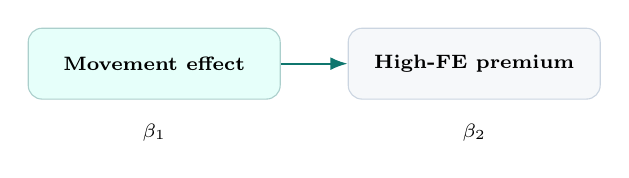
\begin{tikzpicture}
\node[draw=AccentTeal!35,fill=SoftTeal,rounded corners=5pt,minimum width=3.2cm,minimum height=0.9cm,font=\scriptsize\bfseries] (m) {Movement effect};
\node[draw=LineGray,fill=SoftGray,rounded corners=5pt,minimum width=3.2cm,minimum height=0.9cm,font=\scriptsize\bfseries,right=0.85cm of m] (h) {High-FE premium};
\draw[-{Latex[length=2.2mm]},thick,AccentTeal] (m) -- (h);
\node[below=0.18cm of m,font=\scriptsize] {$\beta_1$};
\node[below=0.18cm of h,font=\scriptsize] {$\beta_2$};
\end{tikzpicture}
\end{center}

\end{frame}

%----------------------------------
\begin{frame}{Behavioral Results: Treatment Defined by log\_quant FE}

\begin{columns}[T,onlytextwidth]
\begin{column}{0.67\textwidth}
\scriptsize
\begin{center}
\rowcolors{2}{SoftGray}{white}
\begin{tabular}{l c c c c}
\toprule
Outcome & $\beta_1$ (post) & $\beta_2$ (post $\times$ high) & Mean & SD \\
\midrule
Absence             & 0.0020   & -0.0082  & 0.004 & 0.066 \\
& (0.0027) & (0.0059) & & \\
Days absent         & 0.0079    & -0.0367 & 0.019 & 0.306 \\
& (0.0123) & (0.0266) & & \\
Overtime            & 0.0777*** & -0.0094  & 0.766 & 0.423 \\
& (0.0122) & (0.0146) & & \\
Turnover            & 0.0035***  & 0.0035* & 0.009 & 0.094 \\
& (0.0010) & (0.0018) & & \\
Changed modal  & -0.0217***  & 0.0270** & 0.762 & 0.426 \\
start hour & (0.0081) & (0.0117) & & \\
\bottomrule
\end{tabular}
\end{center}
\footnotesize
Overtime: Worked more than 8 hours a shift. \\
Standard errors in parentheses. \\
$^{*} p<0.10$, $^{**} p<0.05$, $^{***} p<0.01$. \\
Plant FE used to define treatment: log\_quant. \\
$N = 112{,}623$ (112,290 for on-time).
\end{column}
\begin{column}{0.30\textwidth}
\softbox{tealbox}{%
\coefchartBehaviorLogQuant
}
\end{column}
\end{columns}

\end{frame}

\begin{frame}{Behavioral Effects: Interpretation}

\begin{columns}[T,onlytextwidth]
\begin{column}{0.55\textwidth}
\softbox{bluebox}{%
\textbf{Results show:}
\vspace{0.5cm}

\begin{itemize}
        \item Movement to other plant generates changes in working time and turnover
        \item Movements to high productive plants are associated with larger increase in turnover:
        \begin{itemize}
            \item High-productive plants change modal shifts more frequently than low-productive plants
        \end{itemize}
\end{itemize}
}
\end{column}
\begin{column}{0.41\textwidth}
\softbox{goldbox}{%
Given the excess in working time and modal shift changes in high-productive plants, this could lead to a burden on workers that increases their turnover. 
}
\vspace{0.35cm}
\begin{center}
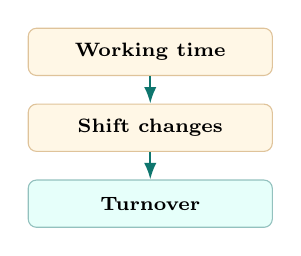
\begin{tikzpicture}[node distance=0.35cm]
\node[draw=AccentGold!45,fill=SoftGold,rounded corners=3pt,font=\scriptsize\bfseries,minimum width=3.1cm,minimum height=0.6cm] (a) {Working time};
\node[draw=AccentGold!45,fill=SoftGold,rounded corners=3pt,font=\scriptsize\bfseries,below=of a,minimum width=3.1cm,minimum height=0.6cm] (b) {Shift changes};
\node[draw=AccentTeal!45,fill=SoftTeal,rounded corners=3pt,font=\scriptsize\bfseries,below=of b,minimum width=3.1cm,minimum height=0.6cm] (c) {Turnover};
\draw[-{Latex[length=2.1mm]},thick,AccentTeal] (a) -- (b);
\draw[-{Latex[length=2.1mm]},thick,AccentTeal] (b) -- (c);
\end{tikzpicture}
\end{center}
\end{column}
\end{columns}

\end{frame}

%----------------------------------
\begin{frame}{Conclusion}

\softbox{bluebox}{%
\textbf{Main result}

\begin{itemize}
\item Moving between plants improve workers productivity 
\item Moving to high-productivity plants do not generate additional gains in workers productivity
\item Moving between plants generate an increase in working time and turnover. 
\item Moving to high-productivity plants generates an excess of worker's burden through more working time and shift changes, producing even larger effects on turnover. 

\end{itemize}
}

\vspace{0.45cm}
\begin{center}
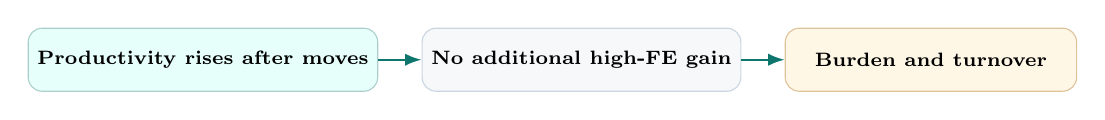
\begin{tikzpicture}[node distance=0.5cm]
\node[draw=AccentTeal!35,fill=SoftTeal,rounded corners=5pt,minimum width=3.7cm,minimum height=0.8cm,font=\scriptsize\bfseries] (a) {Productivity rises after moves};
\node[draw=LineGray,fill=SoftGray,rounded corners=5pt,minimum width=3.7cm,minimum height=0.8cm,font=\scriptsize\bfseries,right=0.55cm of a] (b) {No additional high-FE gain};
\node[draw=AccentGold!45,fill=SoftGold,rounded corners=5pt,minimum width=3.7cm,minimum height=0.8cm,font=\scriptsize\bfseries,right=0.55cm of b] (c) {Burden and turnover};
\draw[-{Latex[length=2.1mm]},thick,AccentTeal] (a) -- (b);
\draw[-{Latex[length=2.1mm]},thick,AccentTeal] (b) -- (c);
\end{tikzpicture}
\end{center}

\end{frame}

%----------------------------------
\begin{frame}{Productivity Results: Treatment Defined by log\_avgtime FE}

\begin{columns}[T,onlytextwidth]
\begin{column}{0.62\textwidth}
\small
\begin{center}
\rowcolors{2}{SoftGray}{white}
\begin{tabular}{l c c}
\toprule
Outcome & $\beta_1$ (post) & $\beta_2$ (post $\times$ high) \\
\midrule
log\_avgtime        & -0.0496*** (0.0180) & 0.0359* (0.0201) \\
log\_quant          & 0.0775*** (0.0203)  & -0.0076 (0.0231) \\
log\_value            & 0.0033 (0.0182)    & 0.0330 (0.0207) \\
\bottomrule
\end{tabular}
\end{center}

\vspace{0.2cm}

\footnotesize
Standard errors in parentheses. \\
$^{*} p<0.10$, $^{**} p<0.05$, $^{***} p<0.01$. \\
Plant FE used to define treatment: log\_avgtime. \\
$N = 112{,}623$.
\end{column}
\begin{column}{0.34\textwidth}
\softbox{tealbox}{%
\coefchartAvgtimeProductivity
}
\end{column}
\end{columns}

\end{frame}

\begin{frame}{Behavioral Results: Treatment Defined by log\_avgtime FE}

\begin{columns}[T,onlytextwidth]
\begin{column}{0.67\textwidth}
\scriptsize
\begin{center}
\rowcolors{2}{SoftGray}{white}
\begin{tabular}{l c c c c}
\toprule
Outcome & $\beta_1$ (post) & $\beta_2$ (post $\times$ high) & Mean & SD \\
\midrule
Absence             & -0.0007    & -0.0015 &  0.004 & 0.066 \\
& (0.0036) & (0.0052) & & \\
Days absent         & -0.0036    & -0.0079 & 0.019 & 0.306 \\
& (0.0145) & (0.0223) & & \\
Overtime            & 0.0774***  & -0.0060 & 0.766 & 0.423 \\
& (0.0127) & (0.0150) & & \\
Turnover            & 0.0072***   & -0.0032* & 0.009 & 0.094 \\
& (0.0018) & (0.0019) & & \\
Changed modal   & -0.0018    & -0.0114 & 0.762 & 0.426 \\
start hour & (0.0106) & (0.0124) & & \\
\bottomrule
\end{tabular}
\end{center}
\footnotesize
Overtime: Worked more than 8 hours a shift. \\
Standard errors in parentheses. \\
$^{*} p<0.10$, $^{**} p<0.05$, $^{***} p<0.01$. \\
Plant FE used to define treatment: log\_avgtime. \\
$N = 112{,}623$ (112,290 for on-time).
\end{column}
\begin{column}{0.30\textwidth}
\softbox{tealbox}{%
\coefchartAvgtimeBehavior
}
\end{column}
\end{columns}

\end{frame}

\end{document}
